\documentclass[12pt,a4paper]{article}
\usepackage[utf8]{inputenc}
\usepackage{amsmath}
\usepackage{amsfonts}
\usepackage{amssymb}
\usepackage{graphicx}
\usepackage[spanish]{babel} 
\usepackage[fixlanguage]{babelbib}
\usepackage[none]{hyphenat}
\usepackage[hidelinks]{hyperref}
\usepackage{titlesec}
\usepackage{titling} 
\usepackage{smartdiagram}
\usepackage{multicol} 
\usepackage{appendix}
\usepackage{tikz}
\usepackage{subfig}
\usetikzlibrary{positioning}
\usepackage{listings,xcolor}
\usetikzlibrary {positioning}
\definecolor {processblue}{cmyk}{0.96,0,0,0}
\selectbiblanguage{spanish}

%\setlist[itemize]{noitemsep}
%\usetikzlibrary{shapes.symbols}
%\usepackage[hmarginratio=1:1,top=32mm,columnsep=20pt]{geometry}
\setlength{\parskip}{2mm}
%\tikzset{description title/.append style={
%		signal, 
%		signal to=south, 
%		signal from=north,
%		yshift=-0.65cm,
%	}
%}
\lstset{
	string=[s]{"}{"},
	stringstyle=\color{blue},
	comment=[l]{:},
	commentstyle=\color{black},
}


\makeatletter
\newenvironment{code}
{\RecustomVerbatimEnvironment{Verbatim}{BVerbatim}{}%
	\def\FV@BProcessLine##1{%
		\hbox{%
			\hbox to\z@{\hss\kern\FV@NumberSep}%
			\FancyVerbFormatLine{##1}%
		}%
	}%
	\VerbatimEnvironment
	\setbox\z@=\hbox\bgroup
	\begin{minted}{js}}
	{\end{minted}\egroup
	\leavevmode\vbox{\hrule\kern2mm\box\z@\kern2mm\hrule}}
\makeatother

\title{PEC 2}


\setlength{\droptitle}{-5\baselineskip} % Move the title up
\pretitle{\begin{center}\Huge\bfseries} % Article title formatting
	\posttitle{\end{center} \vspace{-15pt}} % Article title closing formatting



\title{Práctica II\\Tipología \\ y \\Ciclo de Vida de los datos \\} % Article title
\author{%
		\protect
\includegraphics[trim = 0mm 0mm 0mm 0mm, clip,scale=0.3]{images/uoc}\\ %53 en 3 quito titulo
	\textsc{Gregorio Andrés García Menéndez} \\ % Your name
	\textsc{ Manuel Gómez Montero}
		%\normalsize \href{mailto:mnlgmontero@uoc.edu}{mnlgmontero@uoc.edu}  
% Your email address
	%\and % Uncomment if 2 authors are required, duplicate these 4 lines if more
	%\textsc{Jane Smith}\thanks{Corresponding author} \\[1ex] % Second author's name
	%\normalsize University of Utah \\ % Second author's institution
	%\normalsize \href{mailto:jane@smith.com}{jane@smit\clearpageh.com} % Second author's email address
}
\date{\today} % Leave empty to omit a date
%\renewcommand{\maketitlehookd}{%

\makeindex
\begin{document}
	\nocite{*}
	\maketitle
\tableofcontents
\clearpage

\section{Introducción}

\subsection{Objetivos}
El objetivo de esta práctica es aplicar los conocimientos ... bla bla bla.... 


\subsection{Descripción del Dataset}
El dataset escogido ha sido obtenido a través de una encuesta de estudiantes de secundaria que asisten a cursos de matemáticas y  portugués. Este conjunto de datos contiene bastante información de interés sobre los estudiantes. 

Los datos han sido obtenidos de \textit{Kaggle} y se encuentran en dos ficheros independientes, cada uno de estos ficheros contiene las siguientes variables: 

\begin{enumerate}
	\item \textit{school}: Define la escuela del estudiante. Puede ser ``GP'' (Gabriel Pereira) o ``MS'' (Mousinho da Silveira).
	\item \textit{sex}: Indica el sexo del estudiante.
	\item \textit{age}: Se refiere a la edad del estudiante.
	\item \textit{address}: Indica si el estudiante vive en zona urbana o rural.
	\item \textit{famsize}: Define si la familia se compone de menos de tres miembros o de tres o más.
	\item \textit{Pstatus}: Se refiere al estado de los padres, si viven juntos o no.
	\item \textit{Medu}: Nivel de educación de la madre (0: Ninguna, 1: Primaria (hasta 4º), 2: Primaria (Desde 5º), 3: Secundaria o  4: Educación superior).
	\item \textit{Fedu}: Nivel de educación del padre (0: Ninguna, 1: Primaria (hasta 4º), 2: Primaria (Desde 5º), 3: Secundaria o  4: Educación superior).
	\item \textit{Mjob}:  Trabajo de la madre.
	\item \textit{Fjob}: Trabajo del padre.
	\item \textit{reason}: Razón por la que se escoge esta escuela.
	\item \textit{guardian}: Tutor del alumno.
	\item \textit{traveltime}: Tiempo de camino a la escuela  (1: <15 min., 2: 15 to 30 min., 3: 30 min. a 1 hora,4: >1 hora).
	\item \textit{studytime}: Tiempo de estudio semanal ( 1: <2 horas, 2: 2 a 5 horas, 3: 5 a 10 horas o  4: >10 horas).
	\item \textit{failures} - Número de fracasos en clases pasadas (4 para 4 o más)
	\item \textit{schoolsup} - Define si el estudiante recibe o no clases particulares. 
	\item \textit{famsup} - Indica si el estudiante recibe apoyo educativo familiar.
	\item \textit{paid}: Clases extra pagadas dentro de la asignatura del curso. 
	\item \textit{activities}: Actividades extraescolares.
	\item \textit{nursery}: Indica si asistió a la guardería. 
	\item \textit{higher}: Define si el estudiante tiene intención de  realizar estudios superiores.
	\item \textit{internet}: Indica si el estudiante posee internet en casa.
	\item \textit{romantic}: Define si el estudiante tiene una relación amorosa. 
	\item \textit{famrel}: Calidad de las relaciones familiares (De 1 a 5 de peor a mejor).
	\item \textit{freetime}: Indica la cantidad de tiempo libre del estudiante (De 1 a 5 de menos a más).
	\item \textit{goout}: Mide la frecuencia con la que el estudiante sale con amigos (De 1 a 5 de menos a más).
	\item \textit{Dalc} -Consumo de alcohol entre semana (De 1 a 5 de menos a más).
	\item \textit{Walc} - Consumo de alcohol los fines de semana (De 1 a 5 de menos a más).
	\item \textit{health} - Mide el estado de salud del estudiante (De 1 a 5 de peor a mejor).
	\item \textit{absences}: Número de ausencias a clase.
	\item \textit{G1}: Calificación del primer periodo.
	\item \textit{G2}: Calificación del segundo periodo.
	\item \textit{G3}: Calificación final.
\end{enumerate}




\section{Limpieza de datos}
\subsection{Unión de conjuntos}
El primer paso consiste en unir ambos conjuntos de datos para tener un único dataset que será el que utilizaremos en el resto del documento. 

Según se indica en Kaggle existen 382 estudiantes que asisten a ambos cursos y estos estudiantes pueden ser identificados por las siguientes características: colegio, sexo, edad, dirección, tamaño de familia, trabajo y nivel de educación de los padres, razón por la que ha elegido el colegio, si han asistido a la guardería y si poseen internet en casa. 

Sin embargo creemos que además de estas características hay otras que no pueden variar en un mismo estudiante en ambos ficheros como son el tiempo de camino a la escuela, número de fracasos en clases pasadas, si realiza actividades extraescolares, si tiene intención de realizar estudios superiores, si tiene una relación, la calidad de las relaciones, la frecuencia de salidas con amigos, la cantidad consumida de alcohol y el estado de salud. Con esta separación vemos que existen 320 estudiantes que asisten a ambas clases. 

Comparando los valores de ambos cursos del resto del variables vemos que también coinciden en ambos cursos el tutor del alumno, si recibe soporte familiar y el tiempo de estudio. 


 \begin{figure}[ht!]
	\centering
	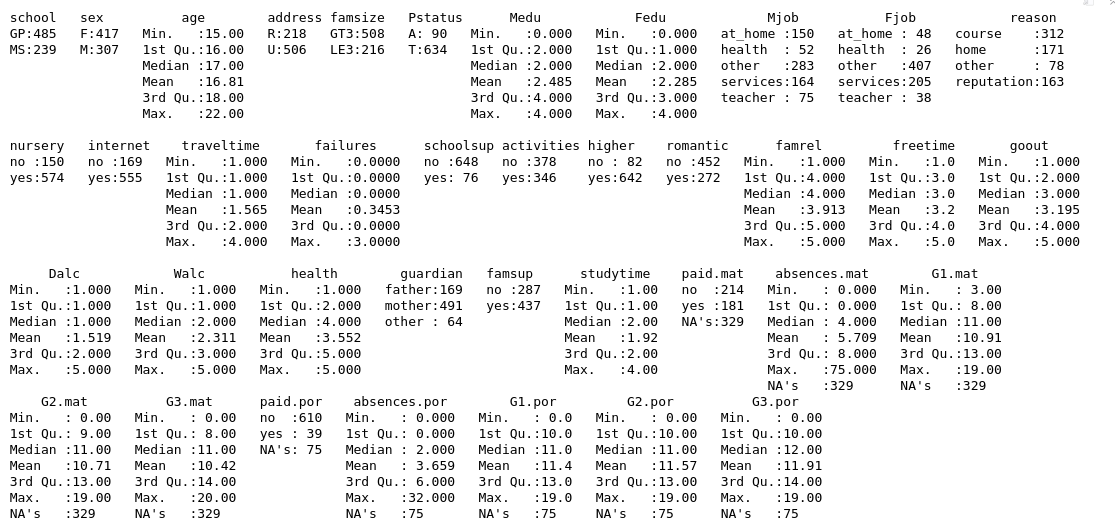
\includegraphics[trim = 0mm 0mm 0mm 0mm, clip,scale=0.4]{images/summary_inicial}
	\caption{Summary dataset conjunto}
	\label{fig:sum1}
\end{figure}


El dataset resultado de la unión posee un total de 724 alumnos 75 de los cuales solo asisten a matemáticas, 329 solo a portugués y  320 a ambos cursos.


\subsection{Tratamiento de NAs}
En primer lugar vamos a encargarnos de los valores perdidos que se dan unicamente en los casos de que los alumnos no hayan asistido a alguno de los cursos, una opción sería eliminar los datos de cualquier alumno que no posea datos en algunos de los cursos, pero implicaría quedarnos solo con un 44\% de los datos. 

Por lo tanto la opción escogida para los valores perdidos es la siguiente: 

\begin{itemize}
	\item \textit{paid}: Unificaremos las variables de ambos cursos tomando un valor ``yes'' cuando el alumno de clases extras pagadas de alguno de los cursos. 
	\item \textit{absences}: Viendo los números parece que las ausencias son mayores en matemáticas. Como lo que nos interesa es saber los alumnos que han faltado más o menos y queremos evitar que tenga un mayor peso los alumnos de matemáticas. Normalizaremos estos valores y en el caso de que los alumnos hayan asistido a ambos cursos utilizaremos la media de ambos valores.
	 \item \textit{calificaciones}: En este caso todas las calificaciones se mueven en el mismo rango por lo que en el caso de los alumnos que hayan asistido a ambos cursos aplicaremos la media de ambos. 
\end{itemize}
 \begin{figure}[ht!]
	\centering
	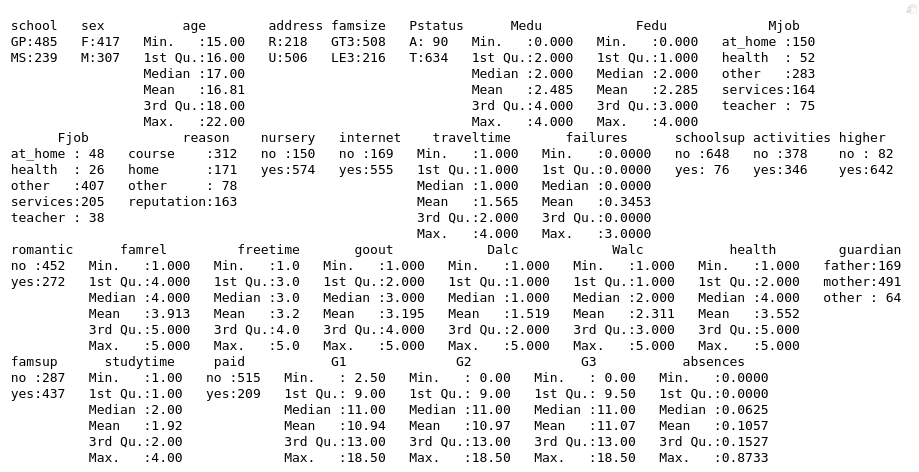
\includegraphics[trim = 0mm 0mm 0mm 0mm, clip,scale=0.4]{images/summary_nonas}
	\caption{Summary dataset sin NAs}
	\label{fig:sum2}
\end{figure}



En el notebook se pueden ver los detalles de estos procesos en la figura \ref{fig:sum2} podemos ver la salida del comando \textit{summary} para este nuevo dataset.



\subsection{Selección de variables/Reducción de dimensionalidad}
Observando el dataset vemos que, aún tras la unión de los datasets, tenemos una gran cantidad de dimensiones, en concreto 33, lo que puede dificultar nuestro análisis. En esta primera fase vamos a hacer una primera aproximación para reducir la dimensionalidad. Posteriormente en los primeros apartados del análisis estadístico reduciremos aún más esta dimensionalidad.

En primer lugar existen variables que, a priori, tienen poca significancia para nuestro análisis como puede ser la escuela a la que asiste el alumno, por lo que podemos eliminar esta variable. 

Por otro lado podemos agrupar las calificaciones en una única variable que nos indique la calificación media del alumno. 

Con estos detalles que pueden observarse en el notebook vemos que hemos conseguido reducir a 30 la dimensionalidad.


\begin{figure}[ht!]
\centering
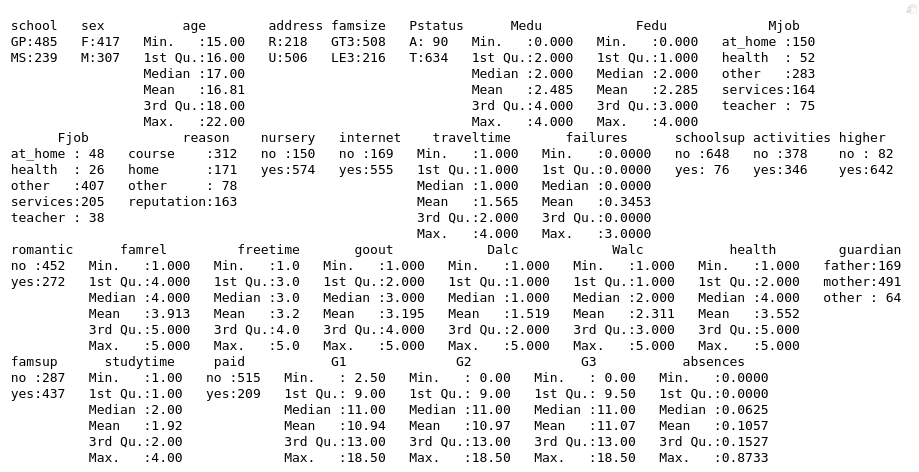
\includegraphics[trim = 0mm 0mm 0mm 0mm, clip,scale=0.4]{images/summary_nonas}
\caption{Summary dataset reducido}
\label{fig:sum3}
\end{figure}






\subsection{Tipos de Variables}
En los tipos mostrados hay algunos que no es correcto el tipo. En la educación tanto de la madre como del padre consideramos que aunque se use un número para la representación debería ser un factor. Lo mismo ocurre para el tiempo de viaje o el tiempo de estudio.  Podemos encontrar más detalles en el notebook. 

\section{Análisis Estadístico}
\subsection{Análisis gráfico inicial}
Observando las gráficas vemos que hay variables que parece que sí tienen influencia a simple vista en el consumo de alcohol tanto a diario como los fines de semana como pueden ser el sexo, el estado de los padres, sin embargo vemos otros que, a priori, no parece que tengan influencia así que en un primer momento vamos a dejar fuera del análisis si el alumno tiene internet, si tiene una relación, el tutor, la dirección, si realiza actividades extraescolares, si recibe clases de pago o si  recibe el apoyo de su familia en el estudio. 

TODO meter algunas de las gráficas 

\begin{figure}[ht!]
	\centering
	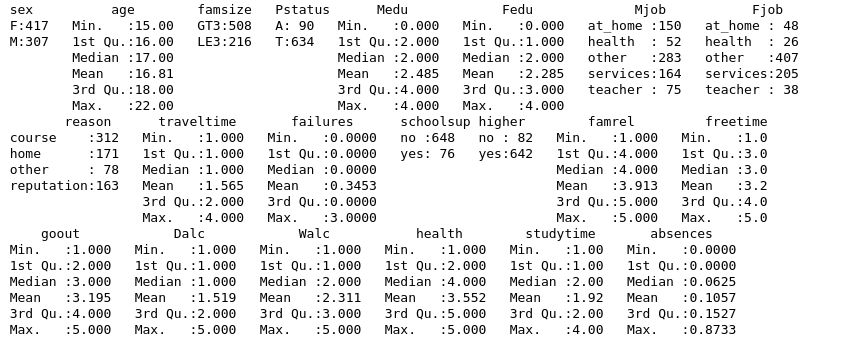
\includegraphics[trim = 0mm 0mm 0mm 0mm, clip,scale=0.4]{images/summary_final}
	\caption{Summary dataset final}
	\label{fig:sum4}
\end{figure}


En la figura \ref{fig:sum4} podemos ver el resumen del dataset. Tras la fase de limpieza y este pequeño análisis hemos pasado de tener dos datasets con 33 dimensiones a \textbf{un único dataset con 21 dimensiones} pasando por un dataset conjunto de 41 dimensiones.  



\subsection{ Estadística Inferencial}
En este apartado vamos a ver si hay diferencia significativas en el consumo de alcohol a diario o fines de semana entre estudiantes de distinto sexo o entre estudiantes con diferente situación de los padres. 


\section{Conclusiones}


\newpage
\bibliography{biblio} 
\bibliographystyle{alphadin} 



	
\end{document} x